%!TEX root = thesis.tex

\chapter{Methoden} % (fold)
\label{cha:methoden}

\section{Graphen} % (fold)
\label{sec:graphen}
Da die Breitensuche ein asymptotisch relativ schneller Algorithmus ist, sind relativ große Testgraphen nötig, um einigermaßen aussagekräftige Ergebnisse zu produzieren. Für diese Arbeit wurden Graphen in der Größenordnung von 100 000 Knoten gewählt. Diese wiederum relativ kleine Ausdehnung wurde gewählt, da der Testmodus beinhaltet, dass bei gleichbleibender Knotenanzahl die Dichte des Graphen variiert. Sehr dicht besiedelte Graphen mit 100 000 Knoten passen gerade noch in den Arbeitsspeicher. Würden noch größere Graphen verwendet, müsste entweder die Dichte des Graphen beschränkt werden oder das Betriebssysteme müsste Daten auslagern, was die Messergebnisse unbrauchbar machen würde. Da die asymptotische Laufzeit der Breitensuche aber O(n + m) ist \cite{SWB-283374373}, ist zu erwarten, dass bei gleicher (absoluter) Kantenzahl und erhöhter Knotenzahl, die Laufzeit identisch ist. Ein Beispiel: BFS auf einem Graph mit 100 000 Knoten und durchschnittlichem Knotengrad von 1000 (ergibt 100 Mio Kanten) dauert gleichlang wie die BFS auf einem Graph mit 1 000 000 Knoten und durchschnittlichem Knotengrad von 100 (ergibt ebenso 100 Mio Kanten).

Es wurde ein Tool namens graph-generator \cite{graph-generator:2009:Online} eingesetzt, um zufällige Graphen zu generieren. Wie gesagt wurde als Knotenanzahl konstant 100 000 gewählt. Um einen Graph zu erstellen werden folgende Parameter gewählt:
\begin{description}
	\item[Minimaler Knotengrad min = 1] Der minimale Ausgangsgrad jedes Knotens.
	\item[Maximaler Knotengrad $max = \infty$] Der maximale Ausgangsgrad jedes Knotens.
	\item[Exponent exp = 5] Der Exponent der Exponentialverteiltung
	\item[Mittlerer Knotengrad z variiert]
\end{description}
Der Ausgangsgrad der Knoten ist folgendermaßen verteilt:
$$
P(X=k) \propto (k + offset)^{-exp}
$$
Der Offset wird dabei automatisch von dem Tool so gewählt, dass sich ein durchschnittlicher Ausgangsgrad von z ergibt.
% section graphen (end)

\section{Testplattformen} % (fold)
\label{sec:testplattform}
\begin{description}
	\item[Testplattform 1] Als Testplattform kann ein Apple Notebook von 2011 zum Einsatz. Es hat einen Intel Core i7-2720QM \enquote{Sandy Bridge} Prozessor, der mit 2.2Ghz getaktet wird. Es stehen 4 physikalische Kerne zur Verfügung, die jeweils Intels Hyper Threading Technologie unterstützen. Dadurch sind physikalisch 8 parallel laufende Threads möglich. Für den Vergleich sequentieller Algorithmen mit parallelen ist zu beachten, dass der Prozessor einen Kern auf bis zu 3.3 GHz übertakten kann, falls die anderen Kerne momentan nicht verwendet werden. Der optimal erreichbare Speedup ist demnach nicht 8.0, sondern deutlich darunter. Das Testsystem ist außerdem mit 8GB Hauptspeicher ausgestattet, der mit 1333MHz, der bei einem Takt von 1333Mhz arbeitet. Auf dem Testsystem wird als Betriebssystem Mac OS X 10.6.8 \enquote{Snow Leopard} und der x10 Compiler in der Version 2.2.3 verwendet.
	\item[Testplattform 2] Als zweiter Testrechner kam ein Desktop mit einem Intel Core i3-550 zum Einsatz. Die Takrate beträgt hier 3.2 GHz. Es stehen zwei Rechenkerne mit Hyper Threading, also 4 getrennte Ausführungsfäden zur Verfügung. Im System sind 2GB Hauptspeicher installiert. Als Betriebssystem wurde Ubuntu 12.04 verwendet. Der x10 Compiler wurde in der Version 2.2.3 verwendet. 

\end{description}
% section testplattform (end)

\section{Modus} % (fold)
\label{sec:modus}
Um Ergebnisse aus je einer Algorithmus - Graph - Kombination zu erhalten, wird der gewählte Algorithmus 3 mal auf dem gewählten Graph ausgeführt und die Zeit gemessen, die die reine Berechnung benötigte. Die Zeit, um den Graph in den Speicher einzulesen und die Daten auf die Places aufzuteilen, wurde nicht gemessen, da sie wenig mit dem Algorithmus und x10 zu tun hat. Die Zeit, die benötigt wird, um das Ergebnis von den beteiligten Places zurück zum Ursprungsplace zu holen, wird allerdings mitgemessen.

Wird ein x10 Programm mit der Umgebungsvariablen X10\_NPLACES gesetzt ausgeführt, werden die einzelnen Places durch Prozesse (nicht Threads) simuliert. Der Aufbau entspricht zwar nicht ganz dem Optimalsetup, in dem jeder Place einen physikalisch getrennten Speicherbereich repräsentiert, doch auch der Kontextwechsel, der bei der Kommunikation zwischen Places auftritt, ist relativ langsam und somit eine Annäherung an realen Kommunikationsoverhead. Trotzdem sind diese Ergebnisse nicht eins zu eins auf einen Rechnerverbund zu übertragen. Zum einen liegt das daran, dass, wie gesagt, die Kommunikation nochmal erheblich teurer wird, zum anderen können mit einem Rechnerverbund wesentlich größere Graphen bearbeitet werden, die offensichtlich ein viel höheres Potential zur Parallelisierung bieten. Andererseits dürfen die Ergebnisse dieser Arbeit auch nicht mit der lokalen Parallelisierung der Breitensuche auf einem einzelnen Rechner verwechselt werden. Kommunikation mittels geteiltem Speicher ist deutlich schneller, als die hier verwendete Inter-Prozess-Kommunikation. \\
Um die Möglichkeit der Parallelität zu messen, wurde der Algorithmus in der 1D und der 2D Zerlegung jeweils in einer Konfiguration mit 1, 2, 4, 8 und 9 Places ausgeführt. Die Konfiguration mit 9 Places wurden hinzugenommen, da so bei der 2D Zerlegung eine symmetrische 3 mal 3 Zerlegung stattfinden kann. Es wurde vermutet, dass eine quadratische Anzahl an Places besonders günstig für diesen Algorithmus sind. Der Vollständigkeit halber wurde auch der 1D Algorithmus mit 9 Places durchgeführt.

Um vollständige Ergebnisse zu bekommen, sollte eigentlich pro Graph die Breitensuche einmal von jedem Knoten aus gestartet werden. Allein diese Unterfangen würde den Zeitrahmen der kompletten Arbeit sprengen.     
% section modus (end)

\chapter{Ergebnisse und Diskussion} % (fold)
\label{cha:ergebnisse_und_diskussion}

Die vollständigen Messergebnis finden sich in Anhang \ref{Anhang-Messwerte}. Wie bereits in Kapitel \ref{cha:methoden} beschrieben, wurde die Dichte des Graphen bei gleichbleibender Knotenanzahl erhöht. Sehr dünn besetzte Graphen waren deutlich schneller mit einer seriellen Version der Breitensuche zu lösen, als es mit jedwedem parallelen Algorithmus möglich war. Auch bei dichten Graphen war kein paralleler Algorithmus wirklich deutlich schneller. Der Vergleich der seriellen Breitensuche, mit der 1D-Breitensuche mit einem Place ist durchaus auch interessant. Um so mehr Kanten es gab, um so besser hat die 1D-Breitensuche abgeschnitten. Am langsamsten war in jedem Fall die 2D-Breitensuche.

\section{Serieller Fall, 1D mit einem Place und 2D mit einem Place} % (fold)
\label{sec:serieller_fall_vs_1d_mit_einem_place}
Jeder Algorithmus muss pro Iteration jeden aktiven Knoten mindestens einmal anfassen. Außerdem muss jeder Algorithmus pro Iteration jeden der Knoten mindestens einmal anfassen, der von einem der aktiven Knoten aus erreichbar ist. Der serielle Algorithmus tut genau das und nicht mehr. In Tests wurde herausgefunden, dass eine Iteration mittels einer herkömmlichen for-Schleife mit anschließendem direkten Zugriff mittels Index deutlich schneller ist (ca. 30\%), als eine foreach-Schleife. Der 1D-Algorithmus muss pro Iteration die Knoten sortieren (jeden aktiven Knoten einmal anfassen), dann verschicken, was im Fall mit nur einem Place eine einfache Zeigerzuweisung ist, und dann nochmal jeden aktiven Knoten anfassen, um alle erreichbaren Knoten zu erreichen. Der 1D-Algorithmus muss also zweimal über alle aktievn Knoten iterieren, was zumindest theoretisch langsamer sein sollte. Die verwendete optimierte Version legt diese beide Phasen aber zusammen. Zusätzliche Arbeit hat der 1D Algorithmus also nur beim Zurückkopieren des gesamten BFS-Distanz-Arrays. Scheinbar ist der 1D Algorithmus selbst im seriellen Fall schneller, als der serielle Algorithmus. Dass die Laufzeiten bei den kleineren Graphen trotzdem ein Wenig länger sind, liegt daran, dass bei den kleinen Graphen da Zurückkopieren des Arrays ausschlaggebend ist.

Wieso der serielle Algorithmus auf Listenbasis nicht, wie eigentlich erwartet, der schnellste ist, ist nicht ohne weiteres zu erklären. Zufall in Verbindung mit der Garbage Collection sind in Anbetracht der Deutlichkeit der Ergebnisse auszuschließen. Eine mögliche Erklärung ist, dass der Compiler den einen Code besser optimieren konnte, als den anderen, ohne dass sofort offensichtlich ist, woran das liegt.

Wie aus Abbildung \ref{Vergleich_Seriell} hervorgeht, ist der 2D Algorithmus deutlich langsamer als die beiden anderen. Der 2D Algorithmus hat 2 Kommunikationsphasen pro Iteration. In den beiden Phasen wir aber jeweils nur mit $sqrt(p)$ anderen Places kommuniziert (bei p Places), während der 1D Algorithmus potentiell mit allen anderen kommuniziert. Im seriellen Fall ist diese zusätzliche Komplexität natürlich nicht nötig, was den Algorithmus verlangsamt.
% section serieller_fall_vs_1d_mit_einem_place (end)  

\begin{figure}
\centering
\label{Vergleich_Seriell}
\caption{Vergleich der Laufzeiten bei serieller Ausführung, jeweils schnellste gemessene Laufzeit.}
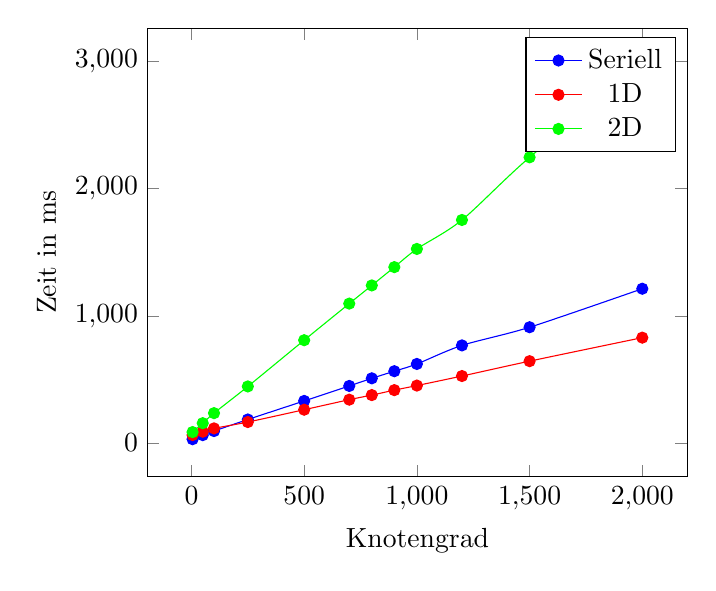
\begin{tikzpicture}
    \begin{axis}[
        xlabel=Knotengrad,
        ylabel=Zeit in ms]
    \addplot[smooth,mark=*,blue] plot coordinates {
        (5,29)
        (50,61)
        (100,93)
        (250,184)
        (500,330)
        (700,448)
        (800,508)
        (900,564)
        (1000,621)
        (1200,767)
        (1500,910)
        (2000,1213)
    };
    \addlegendentry{Seriell}

    \addplot[smooth,color=red,mark=*]
        plot coordinates {
        (5,62)
        (50,88)
        (100,114)
        (250,164)
        (500,261)
        (700,340)
        (800,376)
        (900,415)
        (1000,451)
        (1200,526)
        (1500,643)
        (2000,828)
        };
    \addlegendentry{1D}

    \addplot[smooth,color=green,mark=*]
        plot coordinates {
        (5,85)
        (50,155)
        (100,234)
        (250,444)
        (500,808)
        (700,1096)
        (800,1239)
        (900,1383)
        (1000,1526)
        (1200,1754)
        (1500,2247)
        (2000, 2969)
        };
    \addlegendentry{2D}
    \end{axis}
\end{tikzpicture}
\end{figure}

\section{Ergebnisse der Parallelisierung} % (fold)
\label{sec:ergebnisse_der_parallelisierung}

% section ergebnisse_der_parallelisierung (end)

\section{Die 2D Breitensuche} % (fold)
\label{sec:die_2d_breitensuche}

% section die_2d_breitensuche (end)
% chapter ergebnisse_und_diskussion (end)